\documentclass[a4paper,10pt,fleqn,dvipdfmx]{jsarticle}
%\documentclass[a4paper,10pt,fleqn]{jreport}
%\documentclass[a4paper,10pt,fleqn]{jsbook}

% title
%\title{TeX}
%\date{}

\usepackage[dvipdfm,dvips]{graphicx}
\usepackage{bm}
\usepackage{amsmath,amssymb}
\usepackage{ascmac}
\usepackage{tikz}


\usepackage[dvipdfmx, colorlinks=true, bookmarks=true, bookmarksnumbered=true,
bookmarkstype=toc, linkcolor=blue, urlcolor=blue,
citecolor=blue]{hyperref}
\usepackage{pxjahyper}


\renewcommand{\figurename}{Fig.}

%layout 
\setlength{\topmargin}{-20mm}
\setlength{\textheight}{25.5cm}

\pagestyle{headings}
%%%% end preamble

%%%%%%%%%%%%%%%%%%%%%%%%%%%%%%%%%%%%%%%%%%%%%%%%%%%%%%%%%%%
\begin{document}
%\maketitle

%% report title
\begin{flushleft}
\begin{Large}
圧縮性Navier-Stokes方程式のPISO法による解法
\end{Large}
\end{flushleft}

%% autho
\begin{flushright}
作成 2024/09/13\\
%改訂 XX/XX/XX\\
\end{flushright}

%%%%%%%%%%%%%%%%%%%%%%%%%%%%%%%%%%%%%%%%%%%%%%%%
%%%  本文
%%%%%%%%%%%%%%%%%%%%%%%%%%%%%%%%%%%%%%%%%%%%%%%
\section{概要}
Issaらによる圧縮性Navier-Stokes方程式による解法について述べる。Issaらに
よる論文\cite{Issa1991}--\cite{Issa1986}を参考にした。基礎方程式を有限体
積的に積分した方程式を離散化することで解を求める。

\section{基礎方程式}
ここでは流体は理想気体とし,2次元の圧縮性Navier-Stokes方程式を考える。基礎方程式が以下。
\begin{align}
& \frac{\partial \rho}{\partial t} + \frac{\partial}{\partial x_i}(\rho
 u_i) = 0 \label{eq:mass0}\\
& \frac{\partial \rho u_j}{\partial t} + \frac{\partial}{\partial x_i}(\rho
 u_i u_j) = -\frac{\partial p}{\partial x_j} + \frac{\partial
 \tau_{ij}}{\partial x_i} \label{eq:mom0}\\
& \frac{\partial \rho e}{\partial t} + \frac{\partial}{\partial x_i}(\rho
 u_i e) = \frac{\partial}{\partial x_i}\left(k\frac{\partial T}{\partial
 x_i}\right) - \frac{\partial}{\partial x_i}(pu_i) +
 \frac{\partial}{\partial x_i}(u_j \tau_{ij}) \label{eq:en0}
\end{align}
ここで
$\rho, u, e, p, T$は密度,速度,全エネルギー,圧力,温度である。
状態方程式は
\begin{align}
 p=\rho RT
\end{align}
である。$R$は気体定数(単位の次元は[J/kg K])である。
$\tau_{ij}$は粘性応力テンソルで
\begin{align}
 \tau_{ij} = \mu\left(\frac{\partial u_i}{\partial x_j} + \frac{\partial
 u_j}{\partial x_i} -\frac{2}{3}\delta_{ij}\frac{\partial u_k}{\partial x_k}\right)
\end{align}
全エネルギー$e$は
\begin{align}
 e=C_vT+\frac{1}{2}(u^2+v^2)
\end{align}
で,単位は[J/kg]となる。$C_v$は定積比熱で,比熱比$\gamma$を用いて
\begin{align}
 C_v=\frac{R}{\gamma-1}
\end{align}

2次元の場合,式(\ref{eq:mass0})--(\ref{eq:en0})を書き下すと
\begin{align}
& \frac{\partial \rho}{\partial t} + \frac{\partial}{\partial x}(\rho
 u) + \frac{\partial}{\partial y}(\rho  v) = 0 \label{eq:mass1}\\
%
& \frac{\partial \rho u}{\partial t} + \frac{\partial}{\partial x}(\rho
 u u) + \frac{\partial}{\partial y}(\rho
 u v) = -\frac{\partial p}{\partial x} + \frac{\partial
 }{\partial x} \mu \left(\frac{4}{3}\frac{\partial u}{\partial x} -
 \frac{2}{3}\frac{\partial v}{\partial y}\right) +  \frac{\partial
 }{\partial y} \mu \left(\frac{\partial u}{\partial y} +
 \frac{\partial v}{\partial x}\right) \label{eq:mom1x}\\
%
& \frac{\partial \rho v}{\partial t} + \frac{\partial}{\partial x}(\rho
 u v) + \frac{\partial}{\partial y}(\rho
 v v) = -\frac{\partial p}{\partial y} + \frac{\partial
 }{\partial x}  \mu \left(\frac{\partial u}{\partial y} +
 \frac{\partial v}{\partial x}\right) +  \frac{\partial
 }{\partial y} \mu\left(\frac{4}{3}\frac{\partial v}{\partial y} -
 \frac{2}{3}\frac{\partial u}{\partial x}\right) \label{eq:mom1y}\\
%
& \frac{\partial \rho e}{\partial t} + \frac{\partial}{\partial x}(\rho
 (e+p)u) + \frac{\partial}{\partial y}(\rho
  (e+p)v) 
= \frac{\partial}{\partial x}\left(k\frac{\partial T}{\partial
 x}\right) 
+ \frac{\partial}{\partial y}\left(k\frac{\partial T}{\partial
 y}\right) \nonumber \\
& +  \frac{\partial
 }{\partial x} \left[ \mu u \left(\frac{4}{3}\frac{\partial u}{\partial x} -
 \frac{2}{3}\frac{\partial v}{\partial y}\right) + \mu v\left( \frac{\partial u}{\partial y} +
 \frac{\partial v}{\partial x}\right)
 \right] 
+ \frac{\partial}{\partial y}\left[  \mu u \left(\frac{\partial u}{\partial y} +
 \frac{\partial v}{\partial x}\right) +  \mu v\left(\frac{4}{3}\frac{\partial v}{\partial y} -
 \frac{2}{3}\frac{\partial u}{\partial x}\right)\right] \label{eq:en1}
\end{align}

$p=(\gamma-1)(\rho e - 1/2\rho(u^2+v^2))$より
\begin{align}
 \rho(e+p)=\gamma \rho e-
\frac{\gamma-1}{2}\rho(u^2+v^2)
\end{align}
とかける。

\section{積分と離散化}
\begin{figure}[hbpt]
\centering
\begin{tikzpicture}
  \draw[step=1.5] (-3,-3) grid (4.5,4.5);

 \coordinate [label=right:{P}] (P) at (0.75,0.75);
 \fill (P) circle (2pt);
 \coordinate [label=right:{N}] (N) at (0.75,2.25);
 \fill (N) circle (2pt);
 \coordinate [label=right:{S}] (S) at (0.75,-0.75);
 \fill (S) circle (2pt);
 \coordinate [label=right:{E}] (E) at (2.25,0.75);
 \fill (E) circle (2pt);
 \coordinate [label=right:{W}] (W) at (-0.75,0.75);
 \fill (W) circle (2pt);
 \coordinate [label=right:{EE}] (EE) at (3.75,0.75);
 \fill (EE) circle (2pt);
 \coordinate [label=right:{WW}] (WW) at (-2.25,0.75);
 \fill (WW) circle (2pt);
 \coordinate [label=right:{NN}] (NN) at (0.75,3.75);
 \fill (NN) circle (2pt);
 \coordinate [label=right:{SS}] (SS) at (0.75,-2.25);
 \fill (SS) circle (2pt);

 \coordinate [label=right:{NE}] (NE) at (2.25,2.25);
 \fill (NE) circle (2pt);
 \coordinate [label=right:{SE}] (SE) at (2.25,-0.75);
 \fill (SE) circle (2pt);
 \coordinate [label=right:{NW}] (NW) at (-0.75,2.25);
 \fill (NW) circle (2pt);
 \coordinate [label=right:{SW}] (SW) at (-0.75,-0.75);
 \fill (SW) circle (2pt);

\node(e) at (1.5,0.75) {e};
\node(w) at (0,0.75) {w};
\node(n) at (0.75,1.5) {n};
\node(s) at (0.75,0) {s};

\end{tikzpicture}
\caption{cell coordinate} 
\label{fig}
\end{figure}

$x,y$方向のセル幅を$\Delta x, \Delta y$として,方程式を積分する。すべて
の物理量はセル中央で定義されるものとする。つまりコロケート格子を適用する。質量保
存式(\ref{eq:mass1})を積分すると
\begin{align}
 \int_w^e dx \int_s^ndy \left(\frac{\partial \rho}{\partial t} + \frac{\partial}{\partial x}(\rho
 u) + \frac{\partial}{\partial y}(\rho  v) \right) =0
\end{align}
e, w, n, sは$+x, -x, +y, -y$方向のセル界面をそれぞれ表す。上図参照。時間微分はEuler陰
解法で離散化する。時間刻みは$\Delta t$とする。
\begin{align}
 \frac{\rho - \rho^n}{\Delta t} \Delta x \Delta y 
+ \left(\rho u|_e - \rho u|_w\right)\Delta y 
+ \left(\rho v|_n - \rho v|_s\right) \Delta x = 0  
\end{align}
上付き添字は時間ステップを表すが,n+1ステップの量は添字を省略している。$\rho u|_e$はセル界面e上で定義される量であることを示す。

$x$方向の運動量保存式(\ref{eq:mom1x})の積分では,$\rho uu|_e$が出てくる。
これを次のように離散化する。
\begin{align}
 \rho uu|_e = \rho u|_e \frac{u_P +u_E}{2}
\end{align}
添字$P, E$はそれぞれ着目セルおよびそれに隣接する$+x$方向のセル中央の値を
表している。$-x$方向,$+y$, $-y$方向の隣接セルの値は$W, N, S$で表すとす
る。圧力勾配項の積分は
\begin{align}
 \Delta y(p_e - p_w) = \Delta y \left(\frac{p_P+p_E}{2} -
 \frac{p_P+p_W}{2}\right) = \frac{\Delta y}{2}(p_E-p_W)
\end{align}
となる。

以上を踏まえて,運動量保存式,エネルギー保存式
(\ref{eq:mom1x})--(\ref{eq:en1})を積分し,離散化した式が以下で表される。
なお,$\rho u|_e$の評価には1次精度風上差分,拡散項の評価には2次精度中心
差分を用いる。

$x$方向の運動量式
\begin{align}
  a_Pu_P&=a_E u_E + a_Wu_W + a_N u_N+a_S u_S +S_u +\frac{\Delta x\Delta
 y}{\Delta t}\rho_P^n u_P^n - \frac{\Delta y}{2}(p_E-p_W) \\
 a_E &= \frac{4}{3}\mu_e \frac{\Delta y}{\Delta x} + \max(-\frac{\Delta
 y}{2} \rho u|_e, 0)\\
a_W &=  \frac{4}{3}\mu_w \frac{\Delta y}{\Delta x} + \max(\frac{\Delta
 y}{2} \rho u|_w, 0)\\
 a_N &= \mu_n \frac{\Delta x}{\Delta y} + \max(-\frac{\Delta
 x}{2} \rho v|_n, 0)\\
 a_S &= \mu_s \frac{\Delta x}{\Delta y} + \max(\frac{\Delta
 x}{2} \rho v|_s, 0) \\
a_P &= a_E +a_W + a_N + a_S + \rho_P^n \Delta x \Delta y/\Delta t \\
S_u &= \frac{1}{4} \left[ -\frac{2}{3} (v_{NE}-v_{SE}+v_N-v_S) \mu_e
 + \frac{2}{3}(v_N-v_S+v_{NW}-v_{SW}) \mu_w\right. \nonumber \\
&\left. +(v_E-v_W +v_{NE} -v_{NW} )\mu_n - (v_E-v_W+v_{SE}-v_{SW})\mu_s \right]
\end{align}

$y$方向の運動量式
\begin{align}
  a_Pv_P&=a_E v_E + a_W v_W + a_N v_N+a_S v_S +S_v +\frac{\Delta x\Delta
 y}{\Delta t}\rho_P^n v_P^n - \frac{\Delta y}{2}(p_E-p_W) \\
 a_E &= \mu_e \frac{\Delta y}{\Delta x} + \max(-\frac{\Delta
 y}{2} \rho u|_e, 0)\\
a_W &=  \mu_w \frac{\Delta y}{\Delta x} + \max(\frac{\Delta
 y}{2} \rho u|_w, 0)\\
 a_N &= \frac{4}{3}\mu_n \frac{\Delta x}{\Delta y} + \max(-\frac{\Delta
 x}{2} \rho v|_n, 0)\\
 a_S &= \frac{4}{3}\mu_s \frac{\Delta x}{\Delta y} + \max(\frac{\Delta
 x}{2} \rho v|_s, 0) \\
a_P &= a_E +a_W + a_N + a_S + \rho_P^n \Delta x \Delta y/\Delta t \\
S_v &= \frac{1}{4} \left[ 
(u_{NE}-u_{SE}+u_N-u_S) \mu_e
 - (u_N-u_S+u_{NW}-u_{SW}) \mu_w\right. \nonumber \\
&\left. -\frac{2}{3}(u_E-u_W +u_{NE} -u_{NW} )\mu_n + \frac{2}{3}(u_E-u_W+u_{SE}-u_{SW})\mu_s \right]
\end{align}

エネルギー式
\begin{align}
   a_Pe_P&=a_E e_E + a_W e_W + a_N e_N+a_S e_S +S_e +\frac{\Delta x\Delta
 y}{\Delta t}\rho_P^n e_P^n \\
a_E &= \frac{\Delta y}{\Delta x}\frac{k_e}{C_v} + \max(-\frac{\gamma\Delta
 y}{2} \rho u|_e, 0)\\
a_W &=  \frac{\Delta y}{\Delta x}\frac{k_w}{C_v} + \max(\frac{\gamma\Delta
 y}{2} \rho u|_w, 0)\\
 a_N &= \frac{\Delta x}{\Delta y}\frac{k_n}{C_v} + \max(-\frac{\gamma\Delta
 x}{2} \rho v|_n, 0)\\
 a_S &= \frac{\Delta x}{\Delta y}\frac{k_s}{C_v} + \max(\frac{\gamma\Delta
 x}{2} \rho v|_s, 0) \\
a_P &= a_E +a_W + a_N + a_S + \gamma\rho_P^n \Delta x \Delta y/\Delta t
 +(1-\gamma)\rho_P \Delta x \Delta y/\Delta t\\
S_e &= \Delta y \frac{\gamma-1}{4}\rho u|_e(u_P^2+v_P^2 + u_E^2+v_E^2)
- \Delta y \frac{\gamma-1}{4}\rho u|_w(u_P^2+v_P^2 + u_W^2+v_W^2)
\nonumber \\
& + \Delta x \frac{\gamma-1}{4}\rho v|_n(u_P^2+v_P^2 + u_N^2+v_N^2)
 - \Delta x \frac{\gamma-1}{4}\rho v|_s(u_P^2+v_P^2 + u_S^2+v_S^2)
\nonumber \\
& + \Delta y\left[\mu u \left(\frac{4}{3}\frac{\partial u}{\partial x} -
 \frac{2}{3}\frac{\partial v}{\partial y}\right) + \mu v\left( \frac{\partial u}{\partial y} +
 \frac{\partial v}{\partial x}\right)\right]_e
- \Delta y\left[\mu u \left(\frac{4}{3}\frac{\partial u}{\partial x} -
 \frac{2}{3}\frac{\partial v}{\partial y}\right) + \mu v\left( \frac{\partial u}{\partial y} +
 \frac{\partial v}{\partial x}\right)\right]_w
\nonumber \\
&+ \Delta x\left[\mu u \left(\frac{\partial u}{\partial y} +
 \frac{\partial v}{\partial x}\right) +  \mu v\left(\frac{4}{3}\frac{\partial v}{\partial y} -
 \frac{2}{3}\frac{\partial u}{\partial x}\right)\right]_n
-  \Delta x\left[\mu u \left(\frac{\partial u}{\partial y} +
 \frac{\partial v}{\partial x}\right) +  \mu v\left(\frac{4}{3}\frac{\partial v}{\partial y} -
 \frac{2}{3}\frac{\partial u}{\partial x}\right)\right]_s
\nonumber \\
& + \frac{\Delta y}{2C_v\Delta x}(k_e(u_P^2+v_P^2 - u_E^2 
- v_E^2) -k_w(u_W^2+v_W^2-u_P^2-v_P^2)) 
\nonumber\\
& +\frac{\Delta x}{2C_v\Delta y}(k_n(u_P^2+v_P^2 - u_N^2 
- v_N^2) -k_s(u_S^2+v_S^2-u_P^2-v_P^2)) 
\end{align}

\section{圧力速度の連成}
Issaらによる計算手順に基づいて,圧力速度の連成手順を示す。

\subsection{エネルギー予測}
\begin{align}
 a_Pe_P^* 
= \sum_{nb=E,W,N,S} a_{nb} e_{nb}^* + \frac{\Delta x \Delta y}{\Delta t}\rho^n_P e_P^n
 +S_e
\end{align}
を用いて,エネルギーの予測値$e^*_P$を求める。上付き添字の*は予測値である
ことを示す。これより温度の予測値$T^*$を求める。

\subsection{速度の予測}
\begin{align}
 &a_Pu_P^* 
= \sum_{nb} a_{nb} u_{nb}^* + \frac{\Delta x \Delta y}{\Delta t}\rho^n_P u_P^n
 +S_u - \frac{\Delta y}{2}(p_E^n - p_W^n)\\
 &a_Pv_P^* 
= \sum_{nb} a_{nb} v_{nb}^* + \frac{\Delta x \Delta y}{\Delta t}\rho^n_P v_P^n
 +S_v  - \frac{\Delta x}{2}(p_N^n - p_S^n)
\end{align}
を用いて,流速の予測値$u^*, v^*$を求める。

\subsection{速度の修正}
速度の予測式を以下のように変形する。
\begin{align}
 &\frac{a_P}{\rho^n} \rho^n u_P^* 
= \sum_{nb} a_{nb} u_{nb}^* + \frac{\Delta x \Delta y}{\Delta t}\rho^n_P u_P^n
 +S_u - \frac{\Delta y}{2}(p_E^n - p_W^n)\\
 &\frac{a_P}{\rho^n}\rho^n v_P^* 
= \sum_{nb} a_{nb} v_{nb}^* + \frac{\Delta x \Delta y}{\Delta t}\rho^n_P v_P^n
 +S_v  - \frac{\Delta x}{2}(p_N^n - p_S^n)
\end{align}
速度の修正式を以下のようにする。
\begin{align}
 &\frac{a_P}{\rho^n} \rho^* u_P^{**} 
= \sum_{nb} a_{nb} u_{nb}^* + \frac{\Delta x \Delta y}{\Delta t}\rho^n_P u_P^n
 +S_u - \frac{\Delta y}{2}(p_E^* - p_W^*)\\
 &\frac{a_P}{\rho^n}\rho^* v_P^{**} 
= \sum_{nb} a_{nb} v_{nb}^* + \frac{\Delta x \Delta y}{\Delta t}\rho^n_P v_P^n
 +S_v  - \frac{\Delta x}{2}(p_N^* - p_S^*)
\end{align}

$\widetilde{a_P}=a_P/\rho^n$,圧力の修正量を$p'=p^*-p^n$とすると
\begin{align}
& \rho^*u_P^{**}=\rho^n u_P^* - \frac{1}{\widetilde{a_P}}\frac{\Delta
 y}{2}(p'_E-p'_W) \\
& \rho^*v_P^{**}=\rho^n v_P^* - \frac{1}{\widetilde{a_P}}\frac{\Delta
 x}{2}(p'_N-p'_S)
\end{align}

質量保存式より
\begin{align}
 \frac{\rho^* - \rho^n}{\Delta t} \Delta x \Delta y 
+ \left(\rho^* u^{**}|_e - \rho^* u^{**}|_w\right)\Delta y 
+ \left(\rho^* v^{**}|_n - \rho^* v^{**}|_s\right) \Delta x = 0   
\end{align}

セル界面の値$\rho u|_e$をRhie-Chow補間により求める。
\begin{align}
 \rho u|_e = \frac{\rho u|_P+\rho u|_E}{2} +
 \frac{1}{2}(d_P+d_E)(p_P-p_E) - \frac{1}{4}d_P(p_W-p_E) - \frac{1}{4}d_E(p_P-p_{EE})
\end{align}
ここで$d_P=\Delta y/\widetilde{a_P}_P$, $d_E=\Delta y/\widetilde{a_P}_E$
とする。$\widetilde{a_P}_P, \widetilde{a_P}_E$はセルP,Eでの
$\widetilde{a_P}$である。これより
\begin{align}
\rho^* u^{**}|_e=\rho^n u^*|_e - \frac{1}{2}(d_P+d_E)(p_E'-p_P') 
\end{align}
質量保存式に代入して,整理すると以下の圧力の方程式が得られる。
\begin{align}
& p_P'\left[\frac{\phi(p^n,T^*)}{\Delta t}\Delta x\Delta y + \frac{\Delta y}{2}(d_P+d_E)
 + \frac{\Delta y}{2}(d_P+d_W) + \frac{\Delta x}{2}(d_P+d_N) +
 \frac{\Delta x}{2}(d_P+d_S)\right] \nonumber \\
& = -\Delta y(\rho^n u^*|_e - \rho^n u^*|_w) - \Delta x(\rho^n
 v^*|_n-\rho^n v^*|_s) 
+\frac{\Delta y}{2}(d_P+d_E)p_E' + \frac{\Delta y}{2}(d_P+d_W)p_W'
 \nonumber \\ &+
 \frac{\Delta x}{2}(d_P+d_N)p'_N + \frac{\Delta x}{2}(d_P+d_S)p_S' -
 \frac{p^n}{\Delta t}(\phi(p^n,T^*) - \phi(p^n, T^n))\Delta x\Delta y
\end{align}
%
ここで$ \rho^* = p^*\phi(p^n, T^*)$であり,
\begin{align}
\phi(p^n,T^*) = \frac{1}{RT^*}
\end{align}
である。

圧力方程式から$p',p^*$を求め,密度$\rho^*$を求める。次に速度の修正式より
$u^{**}, v^{**}$を求める。

\subsection{エネルギーの修正}
\begin{align}
 a_Pe_P^{**} 
= \sum_{nb} a_{nb} e_{nb}^* + \frac{\Delta x \Delta y}{\Delta t}\rho^n_P e_P^n
 +S_e
\end{align}
を用いて,エネルギーの修正値$e^{**}_P$を求める。

\subsection{速度の修正}
2回目の速度の修正を行う。
速度の修正式を以下のようにする。
\begin{align}
 &\frac{a_P}{\rho^*} \rho^{**} u_P^{***} 
= \sum_{nb} a_{nb} u_{nb}^{**} + \frac{\Delta x \Delta y}{\Delta t}\rho^n u_P^n
 +S_u - \frac{\Delta y}{2}(p_E^{**} - p_W^{**})\\
 &\frac{a_P}{\rho^*}\rho^{**} v_P^{***} 
= \sum_{nb} a_{nb} v_{nb}^{**} + \frac{\Delta x \Delta y}{\Delta t}\rho^n v_P^n
 +S_v  - \frac{\Delta x}{2}(p_N^{**} - p_S^{**})
\end{align}

質量保存式より
\begin{align}
 \frac{\rho^{**} - \rho^n}{\Delta t} \Delta x \Delta y 
+ \left(\rho^{**} u^{***}|_e - \rho^{**} u^{***}|_w\right)\Delta y 
+ \left(\rho^{**} v^{***}|_n - \rho^{**} v^{***}|_s\right) \Delta x = 0   
\end{align}
圧力の方程式を得るため,$\rho^{**}u^{***}|_e$をRhie-Chow補間により求める。
$\widetilde{a_P^*}=a_P/\rho^{*}$,$d_P^*=\Delta y/\widetilde{a_P^*}_P,
d_E^*=\Delta y/\widetilde{a_P^*}_E$として
\begin{align}
 \rho^{**}u^{***}|_e&=\frac{1}{2}\left[\frac{\sum_{nb}a_{nb}u^{**}_{nb}
 +S_u +(\Delta x\Delta y/\Delta t)\rho^n_P u_P^n}{\widetilde{a_P^*}_P} 
+ \frac{\sum_{nb}a_{nb}u^{**}_{nb}
 +S_u + (\Delta x\Delta y/\Delta t)\rho^n_E
 u_E^n}{\widetilde{a_P^*}_E}\right] \nonumber \\
& - \frac{1}{2}(d_P^*+d_E^*)(p_E^{**}-p_P^{**})
\end{align}
%
これを質量保存式に代入し,以下の圧力式が得られる。
\begin{align}
 & p_P^{**}\left[\frac{\phi(p^*,T^{**})}{\Delta t}\Delta x\Delta y + \frac{\Delta y}{2}(d_P^*+d_E^*)
 + \frac{\Delta y}{2}(d_P^*+d_W^*) + \frac{\Delta x}{2}(d_P^*+d_N^*) +
 \frac{\Delta x}{2}(d_P^*+d_S^*)\right] \nonumber \\
& =  \frac{\rho_P^n}{\Delta t}\Delta x\Delta y+ \frac{\Delta y}{2}(d_P^*+d_E^*)p_E^{**} + \frac{\Delta
 y}{2}(d_P^*+d_W^*)p_W^{**} +  \frac{\Delta x}{2}(d_P^*+d_N^*)p^{**}_N +
 \frac{\Delta x}{2}(d_P^*+d_S^*)p_S^{**} \nonumber \\
& -\frac{\Delta y}{2} \left[\frac{\sum_{nb}a_{nb}u^{**}_{nb}
 +S_u +(\Delta x\Delta y/\Delta t)\rho^n_E u_E^n}{\widetilde{a_P^*}_E} 
- \frac{\sum_{nb}a_{nb}u^{**}_{nb}
 +S_u + (\Delta x\Delta y/\Delta t)\rho^n_W
 u_W^n}{\widetilde{a_P^*}_W}\right] \nonumber \\
& -\frac{\Delta x}{2} \left[\frac{\sum_{nb}a_{nb}v^{**}_{nb}
 +S_v +(\Delta x\Delta y/\Delta t)\rho^n_N v_N^n}{\widetilde{a_P^*}_N} 
- \frac{\sum_{nb}a_{nb}v^{**}_{nb}
 +S_v + (\Delta x\Delta y/\Delta t)\rho^n_S
 v_S^n}{\widetilde{a_P^*}_S}\right] 
\end{align}
%
これより$p^**$を求め$\rho^{**}$が求まる。次に,$u^{***}, v^{***}$を求め
る。

\subsection{エネルギーの修正}
\begin{align}
 a_Pe_P^{***} 
= \sum_{nb} a_{nb} e_{nb}^{**} + \frac{\Delta x \Delta y}{\Delta t}\rho^n_P e_P^n
 +S_e
\end{align}
を用いて,エネルギーの修正値$e^{***}_P$を求める。

\section{境界条件}
セルPの座標を$(i,j)$とすると,本解析では$i=1,\dots, nx+2$, $j=1,\dots,
ny+2$だけ座標点が存在する。流体領域の境界面は$i=1,2$, $i=nx+1, nx+2$,
$j=1,2$, $j=ny+1, ny+2$の中間面とする。そのため,速度,圧力,温度の境界
条件を$i=1$のeの界面,$i=nx+2$のwの界面($i=nx+1$のeの界面),$j=1$のnの界面,$j=ny+2$のsの界
面($j=ny+1$のnの界面)に対して設定する必要がある。例として,$i=1$のeの界面ですべりなしとする場合,$u[1,j]=-u[2,j]$,
$v[1,j]=-v[2,j]$とする。

またこれらの速度の境界条件を圧力の方程式中の$\rho u|_{e, w},\rho
v|_{n,s}$に対しても反映し,圧力の方程式を修正する必要がある。

\section{例題:Shock Tube}
例として,衝撃波管を用いる。解析条件は以下。
\begin{enumerate}
 \item $x$方向10m,$y$方向1m
 \item nx=1000, ny=20,時間刻み$10^{-5}$s 
 \item 流体は空気を想定し,$\gamma=1.4$,分子量$M=0.029$ kg/mol,
       $R=286.6$J/kg K
 \item 初期条件: $x<5$m 圧力$10^5$Pa, 温度348.4K, 速度0m/s; $x>5$m 圧力
       $10^4$Pa,温度278.7K,速度0m/s
\item 境界条件: すべり壁,壁垂直方向圧力勾配なし,断熱
\end{enumerate}

初期状態0sから0.06s (600 step) 後の分布が以下。
\begin{figure}[htbp]
 \centering
 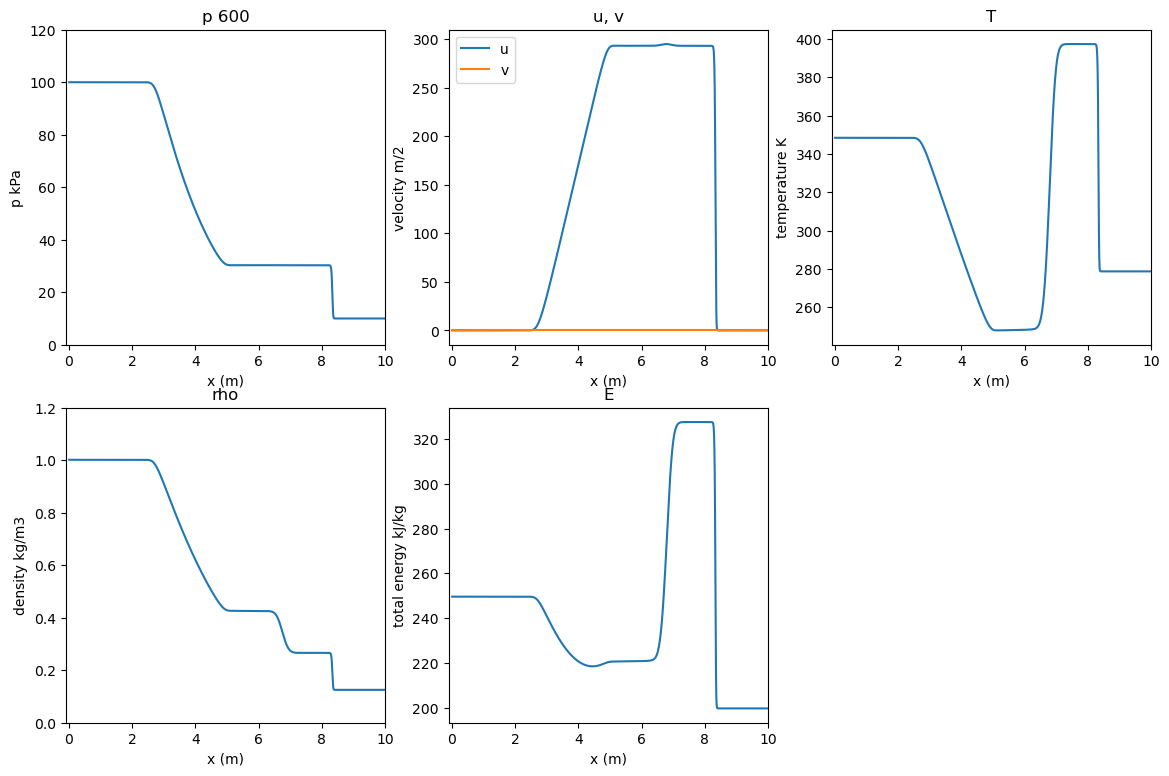
\includegraphics[scale=0.5]{plots_uvTp600.png}
\caption{Pressure, velocity, temperature, density and total energy}
\end{figure}

%% reference
\begin{thebibliography}{99}
\bibitem{Issa1991} R.I. Issa, B. Ahmadi-Befrui, K.R. Beshay, and
        A.D. Gosman, ``Soultion of the Implicityly Discretized Reacting
        Flow Equations by Operator-Splitting'', JCP, (93), pp. 388-410, (1991)
\bibitem{Issa1985} R.I. Issa, ``Solution of the Implicitly Discretised
        Fluid Flow Equations by Operator-Splitting'', JCP, (62),
        pp. 40-65, (1985)
\bibitem{Issa1986} R.I. Issa, A.D. Gosman, and A.P. Watkins, ``The
        Computation of Compressible and Incompressible Recirculating
        Flows by a Non-iterative Implicit Scheme'', JCP, (62),
        pp. 66-82, (1986)
\end{thebibliography}

\end{document}
